\documentclass[../basicOrbitalDynamics.tex]{subfiles}
\graphicspath{{\subfix{../images/}}}
\begin{document}

A plausible scenario for a spacecraft is that telemetry systems provide a distance from the orbited planet and current velocity (as a vector in $\vec{u}_r$ and $\vec{u}_\theta$, noting that $v_n=0$ at all points), while measured or estimated values of $\mu$ would be known. In this case, equations so far derived in terms of geometric values such as $a$ and $e$ will prove widely useless until the precise orbit of the spacecraft is known. Therefore, equations will be derived in terms of these physical values to determine geometric parameters of the orbit. Throughout this chapter, $v$ will be used to refer to the magnitude of $\vv{v}$, while $v_r$ and $v_\theta$, and $\phi$ may also be used. Note that $\phi$ can be found using the fact that $v_\theta=v\cos(\phi)$ so $\phi=\arccos(v_\theta/v)$, with the sign of $\phi$ being the same as the sign of $v_r$.

\bigskip\bigskip
\subsection{Orbit Shape}

Many parameters will depend on the type of orbit that a satellite is in. As such, an easy way of determining this must be found. Section \ref{sec:Specific Energy}, specifically Equation \eqref{Specific Energy Physical} defined specific energy to be
$$\varepsilon=\frac{1}{2}v^2-\frac{\mu}{r}$$

For an orbit to be hyperbolic, the satellite must be able to approach infinite distance from the orbited body, with the velocity always remaining positive. This means the kinetic energy term must be greater in magnitude than the potential energy term, thus making the specific energy positive. For the orbit to be parabolic, the satellite's velocity will approach zero as its distance approaches infinity. This requires the kinetic and potential energy terms to have the same magnitude, making specific energy zero. For a closed orbit, the satellite cannot approach infinite distance without kinetic energy being negative. This means the kinetic term is less than the potential term, making elliptic orbit specific energy negative. This can be summarized with the following statement
\begin{equation}\label{Orbit Shape Physical}
    \text{Orbit Shape}: \begin{cases}
        \text{Elliptic}   & v<\sqrt{\frac{2\mu}{r}} \\
        \text{Parabolic}  & v=\sqrt{\frac{2\mu}{r}} \\
        \text{Hyperbolic} & v>\sqrt{\frac{2\mu}{r}}
    \end{cases}
\end{equation}

Note that it is astronomically (I will not apologize for that) improbable for an orbit to be parabolic, given that there is only one exact state for a parabolic orbit and any deviation from that state will result in an elliptic or hyperbolic orbit.

This can be used to prove an interesting relationship
\begin{align*}
    \varepsilon & = \frac{1}{2}v^2-\frac{\mu}{r}                                     \\
                & = \frac{1}{2}\left(v^2-\frac{\mu}{2r}\right)                       \\
                & = \frac{1}{2}\left(v^2-\left(\sqrt{\frac{\mu}{2r}}\right)^2\right) \\
                & = \frac{1}{2}\left(v^2-\st{v}{escape}^2\right)                    \\
\end{align*}

While this may not be immediately useful, it is nonetheless intriguing.

\bigskip\bigskip
\subsection{Semi-Major Axis}\label{sec:SMA in Terms of V,R}

If $v$ and $r$ are known, Equation \eqref{Vis-Viva Equation} can be solved for $a$.

\begin{align*}
    v                  & = \sqrt{\frac{2\mu}{r}-\frac{\mu}{a}} \\
    v^2                & = \frac{2\mu}{r}-\frac{\mu}{a}        \\
    v^2-\frac{2\mu}{r} & =-\frac{\mu}{a}                       \\
    \frac{\mu}{a}      & = \frac{2\mu}{r}-v^2                  \\
    \frac{a}{\mu}      & = \frac{1}{\frac{2\mu}{r}-v^2}        \\
    a                  & = \frac{\mu}{\frac{2\mu}{r}-v^2}      \\
    a                  & = \frac{\mu r}{2\mu-rv^2}             \\
\end{align*}

Note that $\frac{2\mu}{r}-v^2=\st{v}{escape}^2-v^2$.

\begin{equation}\label{SMA in terms of r, v}
    a=\frac{\mu r}{2\mu-rv^2}=\frac{\mu}{\st{v}{escape}^2-v^2}
\end{equation}

This shows that the semi-major axis of an orbit is inversely proportional to the difference between the squares of escape velocity and current velocity. This also implies that this difference is conserved throughout an orbit.

\bigskip\bigskip
\subsection{Eccentricity}\label{sec:Eccentricity in Terms of V,R}

To determine the eccentricity at any point given $v$, $r$, and $\phi$, angular momentum must be used.

\begin{align*}
    \sqrt{a\mu(1-e^2)}                & =h                                            \\
    \sqrt{a\mu(1-e^2)}                & =rv\cos(\phi)                                 \\
    a\mu(1-e^2)                       & =r^2v^2\cos^2(\phi)                           \\
    \frac{\mu r}{2\mu-rv^2}\mu(1-e^2) & =r^2v^2\cos^2(\phi)                           \\
    \mu(1-e^2)                        & =r^2v^2\cos^2(\phi)\frac{2\mu-rv^2}{\mu r}    \\
    1-e^2                             & =r^2v^2\cos^2(\phi)\frac{2\mu-rv^2}{\mu^2r}   \\
    e^2                               & =1-r^2v^2\cos^2(\phi)\frac{2\mu-rv^2}{\mu^2r} \\
\end{align*}

\begin{equation}
    e=\sqrt{1-r^2v^2\cos^2(\phi)\frac{2\mu-rv^2}{\mu^2r}}
\end{equation}

\bigskip\bigskip
\subsection{Conclusion}

\bigskip
An orbit can take one of three shapes. If the velocity is $v<\sqrt{\frac{2\mu}{r}}$, the orbit is elliptic. If $v=\sqrt{\frac{2\mu}{r}}$ the orbit is parabolic. If the velocity is above escape velocity $v>\sqrt{\frac{2\mu}{r}}$, then the trajectory is be hyperbolic.

\bigskip
The semi-major axis $a$ can be found from measured values
$$a=\frac{\mu r}{2\mu-rv^2}=\frac{\mu}{\st{v}{escape}^2-v^2}$$

\bigskip
The eccentricity is
$$e=\sqrt{1-r^2v^2\cos^2(\phi)\frac{2\mu-rv^2}{\mu^2r}}$$

With the two defining geometric parameters able to be determined from instrumentation readings, equations from Sections \ref{sec:Orbit Geometry} and \ref{sec:Orbital Parameters from Geometry} can be used.

\begin{comment}
\bigskip\bigskip
\subsection{Apsis Radii}
The radii of the apses (periapsis and apoapsis) can be found using a combination of conservation of energy and conservation of angular momentum. The angular momentum at any point is $h=rv_\theta$. Using this, an expression can be found for the radii of the apses (keeping in mind that at periapsis and apoapsis, the velocity is entirely along the horizontal with $\phi=0$).

Beginning with conservation of momentum,
\begin{align*}
    \st{h}{aps}             & = h        \\
    \st{r}{aps}\st{v}{aps} & =rv_\theta \\
\end{align*}
\begin{equation}\label{Apses Radius from h}
    \st{v}{aps}=\frac{rv_\theta}{\st{r}{aps}}
\end{equation}

Switching now to conservation of energy,
\begin{align*}
    \frac{1}{2}\st{v}{aps}^2-\frac{\mu}{\st{r}{aps}} & =\frac{1}{2}v^2-\frac{\mu}{r}                 \\
    \st{v}{aps}^2                                     & =v^2-\frac{2\mu}{r}+\frac{2\mu}{\st{r}{aps}} \\
\end{align*}
\begin{equation}\label{Apses Velocity from Radius}
    \st{v}{aps}=\sqrt{v^2-\frac{2\mu}{r}+\frac{2\mu}{\st{r}{aps}}}
\end{equation}

Setting \eqref{Apses Velocity from Radius} and \eqref{Apses Radius from h} equal to each other,
\begin{align*}
    \frac{rv_\theta}{\st{r}{aps}}       & = \sqrt{v^2-\frac{2\mu}{r}+\frac{2\mu}{\st{r}{aps}}}                            \\
    \frac{r^2v_\theta^2}{\st{r}{aps}^2} & = v^2-\frac{2\mu}{r}+\frac{2\mu}{\st{r}{aps}}                                   \\
    r^2v_\theta^2                        & = v^2\st{r}{aps}^2-\frac{2\mu}{r}\st{r}{aps}^2+2\mu{}\st{r}{aps}              \\
    0                                    & = \left(\frac{2\mu}{r}-v^2\right)\st{r}{aps}^2-2\mu{}\st{r}{aps}+r^2v_\theta^2 \\
\end{align*}

This equation is quadratic in $\st{r}{aps}$ and can be solved
\begin{align*}
    \st{r}{aps} & =\frac{2\mu\pm\sqrt{(2\mu)^2-4(\frac{2\mu}{r}-v^2)(r^2v_\theta^2)}}{2(\frac{2\mu}{r}-v^2)} \\
                 & =\frac{2\mu\pm\sqrt{4\mu^2-4(2\mu{}rv_\theta^2-v^2r^2v_\theta^2)}}{2(\frac{2\mu}{r}-v^2)}  \\
                 & =\frac{2\mu\pm2\sqrt{\mu^2-2\mu{}rv_\theta^2+v^2r^2v_\theta^2}}{2(\frac{2\mu}{r}-v^2)}     \\
                 & =\frac{\mu\pm\sqrt{\mu^2-2\mu{}rv_\theta^2+(rvv_\theta)^2}}{\frac{2\mu}{r}-v^2}            \\
                 & =\frac{\mu{}r\pm{}r\sqrt{\mu^2-2\mu{}rv_\theta^2+(rvv_\theta)^2}}{2\mu-rv^2}               \\
\end{align*}

The substitution will now be made that $v_\theta=v\cos(\phi)$
\begin{align*}
    \st{r}{aps} & =\frac{\mu{}r\pm{}r\sqrt{\mu^2-2\mu{}rv^2\cos^2(\phi)+(rvv\cos(\phi))^2}}{2\mu-rv^2}  \\
                 & =\frac{\mu{}r\pm{}r\sqrt{\mu^2-2\mu{}rv^2\cos^2(\phi)+r^2v^4\cos^2(\phi)}}{2\mu-rv^2} \\
\end{align*}
\begin{equation}\label{Aspes Quadratic Solution}
    \st{r}{aps}=\frac{\mu{}r\pm{}r\sqrt{\mu^2-rv^2(2\mu-rv^2)\cos^2{\phi}}}{2\mu-rv^2}
\end{equation}

A parameter $Q$ will be defined as the square of the ratio between true velocity at any altitude and velocity required for circular orbit at that altitude.
$$Q=(\frac{v}{\sqrt{\mu/r}})^2=\frac{v^2r}{\mu}$$

Solved for $v$, $v=\sqrt{Q\frac{\mu}{r}}$

\begin{align*}
    \st{r}{aps} & =\frac{\mu{}r\pm{}r\sqrt{\mu^2-rv^2\cos^2{\phi}(2\mu-rv^2)}}{2\mu-rv^2}                                                                   \\
                 & =\frac{\mu{}r\pm{}r\sqrt{\mu^2-r(\sqrt{Q\frac{\mu}{r}})^2\cos^2{\phi}(2\mu-r(\sqrt{Q\frac{\mu}{r}})^2)}}{2\mu-r(\sqrt{Q\frac{\mu}{r}})^2} \\
                 & =\frac{\mu{}r\pm{}r\sqrt{\mu^2-Q\mu^2\cos^2{\phi}(2-Q)}}{2\mu-Q\mu}                                                                       \\
                 & =\frac{r\pm{}r\sqrt{1-Q(2-Q)\cos^2{\phi}}}{2-Q}                                                                                           \\
\end{align*}
\begin{equation}\label{Apses Quadratic Solution with Q}
    \st{r}{aps}=\frac{r\pm{}r\sqrt{1-Q(2-Q)\cos^2{\phi}}}{2-Q}
\end{equation}

Equation \eqref{Apses Quadratic Solution with Q} is not in and of itself all that useful, however it allows more exploration of the limitations of Equation \eqref{Aspes Quadratic Solution}.

Equation \eqref{Orbit Shape Physical} can be used to determine how $Q$ depends on the shape of the orbit. For an elliptic orbit $0<Q<2$. For a parabolic orbit $Q=2$. For a hyperbolic orbit, $Q>2$.

In an elliptic orbit where $0<Q<2$, it can be found that $0<Q(2-Q)\cos^2\phi<1$, so $r\sqrt{1-Q(2-Q)\cos^2\phi}$ is strictly positive with magnitude less $r$. Because the denominator is strictly positive, the apoapsis radius is given by the $+$ side of $\pm$ while the periapsis radius is given by the $-$ side.

In a parabolic orbit $Q=2$, making the denominator zero. This means that another method of determining periapsis must be analyzed.

In a hyperbolic orbit in which $Q>2$, $Q(2-Q)\cos^2\phi<0$, so $r\sqrt{1-Q(2-Q)\cos^2\phi}$ is strictly positive with magnitude greater than $r$. Unlike in an elliptic orbit, the denominator will be negative, meaning the numerator should also be negative for a positive (and therefore meaningful) periapsis. This means that, once again, the periapsis is given by the $-$ side of $\pm$.

Equation \eqref{Aspes Quadratic Solution} will be rewritten more concisely as
\begin{equation}\label{Periapsis and Apoapsis Radii}
    [\st{r}{pe}, \st{r}{ap}]=\frac{\mu{}r\mp{}r\sqrt{\mu^2-rv_\theta^2(2\mu{}+rv^2)}}{2\mu-rv^2}
\end{equation}

Note that this equation's results are only as valid is the data inputted+; if bogus data is thrown in, then the result will be equally meaningless. If $v_\theta$ is measured as greater than $v$, then the solution to this equation will have the entire orbit occuring either above or below the measured altitude. Similarly, the apoapsis height for a hyperbola cannot be used for any meaningful analysis, and should be neglected. Finally, this equation will fail to yield any result at all for perfectly parabolic orbits.

\subsubsection{Parabola Periapsis}

The perapsis of a parabolic orbit must be found with different means than that of a hyperbolic or elliptic orbit. Recall from Equation \eqref{Orbit Shape Physical} that in a parabolic orbit, $v=\sqrt\frac{2\mu}{r}$. For angular momentum to be conserved
\begin{align*}
    \st{r}{pe}\st{v}{pe} & =rv_\theta                                         \\
    \st{r}{pe}            & =\frac{rv_\theta}{\st{v}{pe}}                     \\
                           & =\frac{rv_\theta}{\sqrt{\frac{2\mu}{\st{r}{pe}}}} \\
    \st{r}{pe}^2          & =\frac{r^2v_\theta^2}{\frac{2\mu}{\st{r}{pe}}}    \\
    \st{r}{pe}^2          & =\frac{\st{r}{pe}r^2v_\theta^2}{2\mu}             \\
\end{align*}
\begin{equation}\label{Periapsis Radius Parabola}
    \st{r}{pe,parabola}=\frac{r^2v_\theta^2}{2\mu}
\end{equation}

\bigskip\bigskip
\subsection{Velocity as a Function of Radius}

The velocity at any point an in orbit can be found using conservation of energy and momentum. A subscript 0 will be used to signify an initial measurement, to allow clear distinction between $v$, the velocity at any arbitrary point, and $v_0$, the current measured velocity of the satellite.

Conservation of energy will be applied first
\begin{align*}
    \varepsilon                  & =\varepsilon_0                                           \\
    \frac{1}{2}v^2-\frac{\mu}{r} & =\frac{1}{2}v_0^2-\frac{\mu}{r_0}                        \\
    v^2                          & =v_0^2-\frac{2\mu}{r_0}+\frac{2\mu}{r}                   \\
    v                            & =\sqrt{v_0^2-2\mu\left(\frac{1}{r_0}+\frac{1}{r}\right)} \\
\end{align*}

Using conservation of momentum, this can be further expressed as a vector
\begin{align*}
    h         & =h_0                        \\
    rv_\theta & =r_0v_{\theta{}0}           \\
    v_\theta  & =\frac{r_0v_{\theta{}0}}{r} \\
\end{align*}

Knowing that $v^2=v_r^2+v_\theta^2$, the missing component $v_r$ can be found.
\begin{align*}
    v^2                                              & =v_r^2+v_\theta^2                                                                                  \\
    v_0^2-2\mu\left(\frac{1}{r_0}+\frac{1}{r}\right) & =v_r^2+\left(\frac{r_0v_{\theta{}0}}{r}\right)^2                                                   \\
    v_r^2                                            & =v_0^2-2\mu\left(\frac{1}{r_0}+\frac{1}{r}\right)-\left(\frac{r_0v_{\theta{}0}}{r}\right)^2        \\
    v_r                                              & =\sqrt{v_0^2-2\mu\left(\frac{1}{r_0}+\frac{1}{r}\right)-\left(\frac{r_0v_{\theta{}0}}{r}\right)^2} \\
\end{align*}

The velocity vector is therefore
\begin{equation}\label{Velocity Vector}
    \begin{aligned}
        \vv{v} & =\frac{r_0v_{\theta{}0}}{r}\hat{u}_\theta                                                                   \\
               & +\sqrt{v_0^2-2\mu\left(\frac{1}{r_0}+\frac{1}{r}\right)-\left(\frac{r_0v_{\theta{}0}}{r}\right)^2}\hat{u}_r \\
               & +0\hat{u}_n
    \end{aligned}
\end{equation}

Or, written as a magnitude,
\begin{equation}\label{Velocity Magnitude}
    v=\sqrt{v_0^2-2\mu\left(\frac{1}{r_0}+\frac{1}{r}\right)}
\end{equation}


\bigskip\bigskip
\subsection{Flight Path Angle at Any Point}

The simplest expression would be for $\phi$ as a function of $v$, however for the sake of consistency with equations \eqref{Velocity Vector} and \eqref{Velocity Magnitude}, the flight path angle will instead be found as a function of radius. Both $v$ and $v_\theta$, are known, so from trigonometry $\phi$ can be found.

\begin{figure}[H]
    \centering
    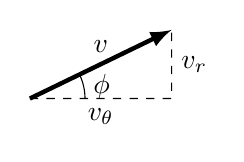
\begin{tikzpicture}[>=latex]
        \def\vel{2}
        \def\velThta{1.8}
        \def\phiAng{\fpeval{acos(\velThta/\vel)}}
        \def\arcRad{0.7}

        \draw[->, ultra thick] (0,0) -- ({deg(\phiAng)}:\vel) node[midway,above] {$v$};
        \draw[dashed] (0,0) -- (\velThta,0) node[midway,below] {$v_\theta$} -- ({deg(\phiAng)}:\vel) node[midway, right] {$v_r$};
        \draw[] (\arcRad,0) arc (0:{deg(\phiAng)}:\arcRad) node[midway, right] {$\phi$};
    \end{tikzpicture}
    \caption{Diagram showing the components of $v$}\label{fig:Velocity Triangle}
\end{figure}

From Figure \ref{fig:Velocity Triangle}, three trigonometric identities can be found.
\begin{align*}
    \cos{\phi}=\frac{v_\theta}{v} \\
    \sin{\phi}=\frac{v_r}{v}      \\
    \tan{\phi}=\frac{v_r}{v_\theta}
\end{align*}

Because the $v$ and $v_\theta$ terms are shortest, the cosine will be used.
\begin{align*}
    \cos(\phi) & = \frac{v_\theta}{v}                                                                 \\
               & = \frac{r_0v_{\theta{}0}/r}{\sqrt{v_0^2-2\mu\left(\frac{1}{r_0}+\frac{1}{r}\right)}} \\
               & = \frac{r_0v_{\theta{}0}}{r\sqrt{v_0^2-2\mu\left(\frac{1}{r_0}+\frac{1}{r}\right)}}  \\
\end{align*}
\begin{equation}\label{Flight Path Angle Physical}
    \phi=\cos^{-1}\left(\frac{r_0v_{\theta{}0}}{r\sqrt{v_0^2-2\mu(\frac{1}{r_0}+\frac{1}{r})}}\right)
\end{equation}

\bigskip\bigskip
\subsection{Geometric Parameters}

Until this point, this section has worked purely with physical quantities instead of the geometric ones already defined. However, it is at this point that geometric identities must be defined in terms of physically measured bases.

\subsubsection{Semi-Major Axis}\label{sec:SMA Physical}

From Figure \ref{fig:Orbit Diagram}, the major axis is the sum of the apoapsis and periapsis radii. Therefore,
\begin{align*}
    2a & = \st{r}{pe}+\st{r}{ap}                                          \\
       & =\frac{\mu{}r-{}r\sqrt{\mu^2-rv_\theta^2(2\mu{}+rv^2)}}{2\mu-rv^2} \\
       & +\frac{\mu{}r+{}r\sqrt{\mu^2-rv_\theta^2(2\mu{}+rv^2)}}{2\mu-rv^2} \\
       & =\frac{2\mu{}r}{2\mu-rv^2}                                         \\
\end{align*}

Dividing both sides by two, this leaves
\begin{align}\label{SMA Physical}
    a = \frac{\mu{}r}{2\mu-rv^2}
\end{align}

An equivalent form of this equation can be found.

\begin{align*}
    a & = \frac{\mu{}r}{2\mu-rv^2}         \\
    a & = \frac{\mu{}}{\frac{2\mu}{r}-v^2}
\end{align*}

Recall from Equation \eqref{Orbit Shape Physical} that escape velocity is $\st{v}{escape}=\sqrt{2\mu/r}$
\begin{align}\label{SMA Physical Escape Velocity}
    a = \frac{\mu{}}{\st{v}{escape}^2-v^2}
\end{align}

This shows that the semi-major axis of an orbit is inversely proportional to the difference between the square of the escape velocity and the current velocity.

\subsubsection{Eccentricity}\label{sec:Eccentricity physical}

Recall from Equation \eqref{Angular Momentum Geometric Definition} that
$$h=\sqrt{a\mu{}(1-e^2)}$$

Equation \eqref{Angular Momentum Physical Definition} adds that
$$h=rv_\perp=rv_\theta$$

These can be set equal to eachother and solved for $e$.
\begin{align*}
    \sqrt{a\mu{}(1-e^2)}                 & = rv_\theta                                       \\
    a\mu{}(1-e^2)                        & = r^2v_\theta^2                                   \\
    \frac{\mu{}r}{2\mu-rv^2}\mu{}(1-e^2) & = r^2v_\theta^2                                   \\
    \frac{\mu^2r}{2\mu-rv^2}(1-e^2)      & = r^2v_\theta^2                                   \\
    1-e^2                                & = \frac{r^2v_\theta^2(2\mu-rv^2)}{\mu^2r}         \\
    e^2                                  & =1-\frac{r^2v_\theta^2(2\mu-rv^2)}{\mu^2r}        \\
    e                                    & =\sqrt{1-\frac{r^2v_\theta^2(2\mu-rv^2)}{\mu^2r}} \\
    e                                    & =\sqrt{1-\frac{rv_\theta^2(2\mu-rv^2)}{\mu^2}}
\end{align*}
\begin{equation}\label{Eccentricity Physical}
    e=\sqrt{1-\frac{rv_\theta^2(2\mu-rv^2)}{\mu^2}} \\
\end{equation}

With both Semi-Major Axis and Eccentricity calculated in terms of physical inputs, any geometric relationships can be expressed in terms of physical inputs. Equations \eqref{SMA Physical} and \eqref{Eccentricity Physical} allow equations such as the orbit equation to be put int terms of physically measured values.

\bigskip\bigskip
\subsection{Period}
Unfortunately, the most efficient way of finding the period from physical inputs is to rewrite Equation \eqref{Period Geometric} from \ref{Sec:Period Geometric} in terms of the semi-major axis found in Section \ref{sec:SMA Physical} (Equation \eqref{SMA Physical}).
\begin{align*}
    P & = \sqrt{\frac{4\pi^2a^3}{\mu}}                          \\
      & = \sqrt{\frac{4\pi^2(\frac{\mu{}r}{2\mu-rv^2})^3}{\mu}} \\
      & = \sqrt{\frac{4\pi^2\mu^3r^3}{\mu(2\mu-rv^2)^3}}        \\
      & = \sqrt{\frac{4\pi^2\mu^2r^3}{(2\mu-rv^2)^3}}           \\
      & = 2\pi\mu\sqrt{\frac{r^3}{(2\mu-rv^2)^3}}               \\
      & = 2\pi\mu\left(\frac{r}{2\mu-rv^2}\right)^{3/2}         \\
\end{align*}
\end{comment}

\end{document}